\section{什么是目标检测}
\begin{frame}[allowframebreaks]
    \frametitle{\textsc{目录}} \vspace{-0.3cm}
    \begin{spacing}{0.0}
        \tableofcontents[currentsection,hideallsubsections]
    \end{spacing}   % 若不想要目录, 注释掉该句
\end{frame}

\begin{frame}
    \noindent\large\textbf{目标检测}
    \vspace{0.4cm}
    \begin{itemize}
        \item[$ \bullet $] 是什么?
        \item[$ \bullet $] 在哪里?
        \item[$ \bullet $] 有哪些?
    \end{itemize}
    \vspace{1cm}
    “是什么”意味着需要判断出找出来的目标是什么,也就是对目标的类别做判断,是人还是狗或者是车\\
    \vspace{1em}
    “在哪里”需要指出找到的目标在图像的那个地方,范围是哪里\\
    \vspace{1em}
    “有哪些”意味着需要将图像当中所有的感兴趣物体(预先定义的类别)找出来\\
\end{frame}

\begin{frame}
    \noindent\large\textbf{如何表示}\\
    在计算机当中需要用数字来表达“是什么”、“在哪里”、“在哪里”
    \vspace{1em}
    \begin{itemize}
        \item[$ \bullet $] 整数(one-hot 向量)表示类别
        \item[$ \bullet $] 矩形框表示位置(四元组$[x,y,w,h]$)
        \item[$ \bullet $] 堆叠所有目标组成数组$n\times5$
    \end{itemize}
    \vspace{1em}
    \begin{figure}
        \subfloat[box]{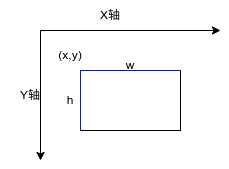
\includegraphics[width=0.4\linewidth]{box.png}}
        \hspace{1cm}
        \subfloat[Object Detection]{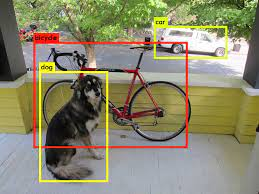
\includegraphics[width=0.4\linewidth]{obd1.jpg}}
    \end{figure}
\end{frame}

\begin{frame}
    \noindent\large\textbf{模型表示}\\
    \vspace{1em}
    知道了如何用数字表达检测结果,那么如何让网络模型输出这些数据?\\
    \vspace{1em}
    \begin{itemize}
        \item[$ \bullet $] 分类表达\\
            \vspace{0.5em}
            对于分类,已经很熟悉了,Softmax计算类别概率就能得到类别\\
            \vspace{0.5em}
        \item[$ \bullet $] 预测框表达\\
            \vspace{0.5em}
            预测框其实是一个四维向量,很容易就能想到用回归来拟合\\
            \vspace{0.5em}
        \item[$ \bullet $] 所有物体表达\\
            \vspace{0.5em}
            所有物体实际上是一个矩阵,是不是也可以用回归来拟合?\\
            \vspace{0.5em}
    \end{itemize}
\end{frame}

\begin{frame}
    \noindent\large\textbf{模型表示}\\
    \vspace{0.5em}
    实际上让神经网络输出所有物体的预测信息是很困难的,因为每张图片当中的物体数量都是不确定的,
    而神经网络无法根据内容调整输出的数量.  \\
    \vspace{0.5em}
    \begin{itemize}
        \item[$ \bullet $] “广撒网,多敛鱼,择优而从之”
            \begin{tabular}{rl}
                广撒网:     & 生成过量的预测框     \\
                多敛鱼:    & 尽可能覆盖所有的目标 \\
                择优而从之: & 询问模型是否存在目标 \\
            \end{tabular}
    \end{itemize}
    通过这种策略,目标检测就变成了“在不在、是什么”的问题
\end{frame}